% !TeX root = ./msb-appendix.tex
\documentclass[alpha-refs]{wiley-article}
\usepackage{siunitx}
\usepackage{microtype}
\usepackage[many]{tcolorbox}
\usepackage{hyperref}
\papertype{}

% Include section in journal if known, otherwise delete
% \paperfield{Journal Section}

\title{Appendix for "Fundamental Limits on the Rate of Bacterial Growth"}

\abbrevs{}

% Include full author names and degrees, when required by the journal.
% Use the \authfn to add symbols for additional footnotes and present addresses, if any. Usually start with 1 for notes about author contributions; then continuing with 2 etc if any author has a different present address.


\author[1\authfn{1}]{Nathan M. Belliveau}
\author[2\authfn{1}]{Griffin Chure}
\author[3]{Christina L. Hueschen}
\author[4]{Hernan G. Garcia}
\author[5]{Jane Kondev}
\author[6]{Daniel S. Fisher}
\author[1,7]{Julie A. Theriot}
\author[8,9]{Rob Phillips}

\contrib[\authfn{1}]{Equally contributing authors.}

% Include full affiliation details for all authors
\affil[1]{Department of biology, University of Washington, Seattle, WA, USA}
\affil[2]{Department of Applied PHysics, California Institute of Technology, Pasadena, CA, USA}
\affil[3]{Department of Chemical ENgineering, Stanford University, Stanford, CA, USA}
\affil[4]{Department of MOlecuular cell Biology and Department of PHysics, University of California Berkeley, Berkeley, CA, USA}
\affil[5]{Department of Physics, Brandeis University, Waltham, MA, USA}
\affil[6]{Department of Applied PHysics, Stanford University, Stanford, CA, USA}
\affil[7]{Allen Institute for Cell Science, Seattle, WA, USA}
\affil[8]{Division of Biology and Biological Engineering, California Institute of Technology, Pasadena, CA, USA}
\affil[9]{Department of Physics, California Institute of Technology, Pasadena, CA, USA}

\corraddress{Julie A. Theriot, University of Washington; Rob Phillips, California Institute of Technology}
\corremail{jtheriot@uw.edu; phillips@pboc.caltech.edu}
\contrib[\authfn{1}]{Equally contributing authors.}

% \fundinginfo{Funder One, Funder One Department, Grant/Award Number: 123456, 123457 and 123458; Funder Two, Funder Two Department, Grant/Award Number: 123459}

% Include the name of the author that should appear in the running header
\runningauthor{Belliveau, Chure et al.}

\begin{document}
\begin{frontmatter}
\maketitle

\end{frontmatter}


\section{Additional Estimates of Fundamental Biological Processes}
\label{sec:SI_nutr_trans}

In the main text of this work, we present estimates for a significant number of
fundamental biological processes that are necessary for cell division. While we
believe the estimates provided in the main text provide a succinct summary of
the corresponding process, we left out additional estimates of related
processes for brevity. In this section of the appendix, we present these
additional estimates in full.


\subsection{Nutrient Transport}
In the main text, we make passing mention that in typical laboratory conditions, transport carbon often
comes in the form of carbohydrates and sugar alcohols while other critical
elements -- such as nitrogen, sulfur, and phosphorus -- are transported as
inorganic ions. Below, we present estimates for the transport requirements of
these materials.

\subsubsection{Nitrogen}
We must first address which elemental sources must require active transport,
meaning that the cell cannot acquire appreciable amounts simply via diffusion
across the membrane. The permeability of the lipid membrane to a large number
of solutes has been extensively characterized over the past century. Large,
polar molecular species (such as various sugar molecules, sulfate, and
phosphate) have low permeabilities while small, non-polar compounds (such as
oxygen, carbon dioxide, and ammonia) can readily diffuse across the membrane.
Ammonia, a primary source of nitrogen in typical laboratory conditions, has a
permeability on par with water ($\sim 10^5$ nm/s, BNID:110824). In
nitrogen-poor conditions, \textit{E. coli} expresses a transporter (AmtB)
which appears to aid in nitrogen assimilation, though the mechanism and
kinetic details of transport are still a matter of debate
\citep{heeswijk2013a, khademi2004}. Beyond ammonia, another plentiful source
of nitrogen come in the form of glutamate, which has its own complex
metabolism and scavenging pathways. However, nitrogen is plentiful in the
growth conditions examined in this work, permitting us to neglect nitrogen
transport as a potential rate limiting process in cell division in typical
experimental conditions.

\subsubsection{Phosphorus}
Phosphorus is critical to the cellular energy economy in the form of
high-energy phosphodiester bonds making up DNA, RNA, and the NTP energy pool as
well as playing a critical role in the post-translational modification of
proteins and defining the polar-heads of lipids. In total, phosphorus
makes up $\approx$3\% of the cellular dry mass which in typical experimental conditions is in the form of inorganic phosphate. The cell membrane
has remarkably low permeability to this highly-charged and critical molecule,
therefore requiring the expression of active transport systems. In \textit{E. coli}, the proton
electrochemical gradient across the inner membrane is leveraged to transport
inorganic phosphate into the cell \citep{rosenberg1977}.
Proton-solute symporters are widespread in \textit{E. coli} \citep{ramos1977,
booth1979} and can have rapid transport rates of 50 to 100 molecules per second for
sugars and other solutes (BNID: 103159; 111777). As a more
extreme example, the proton transporters in the F$_1$-F$_0$ ATP synthase, which
use the proton electrochemical gradient for rotational motion, can shuttle
protons across the membrane at a rate of $\approx$ 1000 per second (BNID:
104890; 103390). In \textit{E.
coli} the PitA phosphate transport system has been shown to be very tightly coupled
with the proton electrochemical gradient with a 1:1 proton:phosphate
stoichiometric ratio \citep{harris2001, feist2007}. Taking the geometric mean of
the aforementioned estimates gives a plausible rate of phosphate transport on
the order of 300  per second. Illustrated in
\textbf{\textit{Figure 2–Figure Supplement 1}}(A), we can estimate that $\approx$ 200
phosphate transporters are necessary to maintain an $\approx$ 3\% dry mass with
a 5000 s division time. This estimate is consistent with observation when we examine the
observed copy numbers of PitA in proteomic data sets (plot in \textbf{\textit{Figure 2–Figure Supplement 1}}(A)). While our estimate is very much in line with the
observed numbers, we emphasize that this is likely a slight overestimate of the
number of transporters needed as there are other phosphorous scavenging systems,
such as the ATP-dependent phosphate transporter Pst system which we have neglected.

\subsubsection{Sulfur}
Similar to phosphate, sulfate is highly-charged and not particularly membrane
permeable, requiring active transport. While there exists a H+/sulfate
symporter in \textit{E. coli}, it is in relatively low abundance and is not
well characterized \citep{zhang2014}. Sulfate is predominantly acquired via
the ATP-dependent ABC transporter CysUWA system which also plays an important
role in selenium transport \citep{sekowska2000, sirko1995}. While specific
kinetic details of this transport system are not readily available, generic
ATP transport systems in prokaryotes transport on the order of 1 to 10
molecules per second (BNID: 109035). Combining this generic transport rate,
measurement of sulfur comprising 1\% of dry mass, and a 5000 second division
time yields an estimate of $\approx$ 1000 CysUWA complexes per cell
(\textbf{\textit{Figure 2–Figure Supplement 1}}(B)). Once again, this estimate is in notable
agreement with proteomic data sets, suggesting that there are sufficient
transporters present to acquire the necessary sulfur. In a similar spirit of
our estimate of phosphorus transport, we emphasize that this is likely an
overestimate of the number of necessary transporters as we have neglected
other sulfur scavenging systems that are in lower abundance.



\subsection{Additional Process of the Central Dogma}
\label{sec:SI_central_dogma}
In the main text, we consider the processes underlying the backbone of the
central dogma, namely DNA replication, RNA transcription, and protein
translation. In this section we turn our attention to additional processes
related to the central dogma, primarily dNTP synthesis for DNA replication and
amino-acyl tRNA synthesis for translation. Additionally, we explore in more
detail the estimates shown in \textbf{\textit{Figure 8}}(A) for the RNA polymerase
requirements of mRNA and tRNA synthesis.

\subsubsection{dNTP synthesis}
The four major dNTPs (dATP, dTTP, dCTP, and dGTP) serve as the fundamental
units of the genetic code. Thus, to faithfully replicate the chromosome, the
cell must be able to synthesize enough of these bases in the first place. All
dNTPs are synthesized \textit{de novo} in separate pathways, requiring
different building blocks. However, a critical step present in all dNTP
synthesis pathways is the conversion from ribonucleotide to
deoxyribonucleotide via the removal of the 3' hydroxyl group of the ribose
ring \citep{rudd2016}. This reaction is mediated by a class of enzymes termed
ribonucleotide reductases, of which \textit{E. coli} possesses two
aerobically active complexes (termed I and II) and a single anaerobically
active enzyme. Due to their peculiar formation of a radical intermediate,
these enzymes have received much biochemical, kinetic, and structural
characterization. One such work \citep{ge2003} performed a detailed
\textit{in vitro} measurement of the steady-state kinetic rates of these
complexes, revealing a turnover rate of $\approx$ 10 dNTP per second.

Since this reaction is central to the synthesis of all dNTPs, it is
reasonable to consider the abundance of these complexes is a measure of the
total dNTP production in \textit{E. coli}. Illustrated schematically in
\textbf{\textit{Figure 7}}(A), we consider the fact that to replicate the cell's
genome, on the order of $\approx 10^7$ dNTPs must be synthesized. Assuming a
production rate of 10 per second per ribonucleotide reductase complex and a
cell division time of 5000 seconds, we arrive at an estimate of $\approx$ 200
complexes needed per cell. As shown in \textbf{\textit{Figure 7–Figure Supplement 1}}, this estimate agrees with the experimental measurements of these
complexes abundances within $\approx 1/2$ an order of magnitude. Extension of
this estimate across a continuum of growth rate, including the fact that
multiple chromosomes can be replicated at a given time, is shown as a grey
transparent line in \textbf{\textit{Figure 7–Figure Supplement 1}}. Similarly to our point estimate, this
refinement agrees well with the data, accurately describing both the
magnitude of the complex abundance and the dependence on growth rate.

Recent work has revealed that during replication, the ribonucleotide
reductase complexes coalesce to form discrete foci colocalized with the DNA
replisome complex \citep{sanchez-romero2011}. This is particularly pronounced
in conditions where growth is slow, indicating that spatial organization and
regulation of the activity of the complexes plays an important role.

\subsubsection{mRNA and tRNA Synthesis}
In \textbf{\textit{Figure 8}} of the main text, we presented
estimates for the number of RNA polymerases needed to synthesize enough mRNA
and tRNA molecules. Here, we present a more detailed rationalization of these estimates.

To form a functional protein, all protein coding genes must first be
transcribed from DNA to form an mRNA molecule. While each protein requires an
mRNA blueprint, many copies of the protein can be synthesized from a single
mRNA. Factors such as strength of the ribosomal binding site, mRNA stability,
and rare codon usage frequency dictate the number of proteins that can be
made from a single mRNA, with yields ranging from 10$^1$ to 10$^4$ (BNID:
104186; 100196; 106254). Computing the geometric mean of this range yields
$\approx$ 1000 proteins synthesized per mRNA, a value that agrees with
experimental measurements of the number of proteins per cell ($\approx 3
\times 10^6$, BNID: 100088) and total number of mRNA per cell ($\approx 3
\times 10^3$, BNID:100064).

This estimation captures the \textit{steady-state} mRNA copy number, meaning
that at any given time, there will exist approximately 3000 unique mRNA
molecules. To determine the \textit{total} number of mRNA that need to be
synthesized over the cell's lifetime, we must consider degradation of the
mRNA. In most bacteria, mRNAs are rather unstable with life times on the
order of several minutes (BNID: 104324; 106253; 111927; 111998). For
convenience, we assume that the typical mRNA in our cell of interest has a
typical lifetime of $\approx$ 300 seconds. Using this value, we can determine
the total mRNA production rate to maintain a steady-state copy number of 3000
mRNA per cell. While we direct the reader to the appendix for a more detailed
discussion of mRNA transcriptional dynamics, we state here that the total
mRNA production rate must be on the order of $\approx$ 15 mRNA per second. In
\textit{E. coli}, the average protein is $\approx$ 300 amino acids in length
(BNID: 108986), meaning that the corresponding mRNA is $\approx$ 900
nucleotides which we will further approximate as $\approx$ 1000 nucleotides
to account for the non-protein coding regions on the 5' and 3' ends. This
means that the cell must have enough RNA polymerase molecules about to
sustain a transcription rate of $\approx 1.5 \times 10^4$ nucleotides per
second. Knowing that a single RNA polymerase polymerizes RNA at a clip of 40
nucleotides per second, we arrive at a comfortable estimate of $\approx$ 250
RNA polymerase complexes needed to satisfy the mRNA demands of the cell. It
is worth noting that this number is approximately half of that required to
synthesize enough rRNA, as we saw in the previous section. We find this to be
a striking result as these 250 RNA polymerase molecules are responsible for
the transcription of the $\approx$ 4000 protein coding genes that are not
ribosome associated.

We now turn our attention to the synthesis of tRNA. Unlike mRNA or rRNA, each
individual tRNA is remarkably short, ranging from 70 to 95 nucleotides each
(BNID: 109645; 102340). What they lack in length, they make up for in
abundance, with reported values ranging from $\approx$5$\times$10$^4$ (BNID:
105280) to $\approx$5$\times$10$^5$ (BNID: 108611). To test tRNA synthesis as
a possible growth-rate limiting stage, we will err towards a higher abundance
of $\approx$ 5$\times$10$^5$ per cell. Combining the abundance and tRNA
length measurements, we make the estimate that $\approx 5 \times 10^7$
nucleotides are sequestered in tRNA per cell. Unlike mRNA, tRNA is remarkably
stable with typical lifetimes \textit{in vivo} on the order of $\approx$ 48
hours \citep{abelson1974,svenningsen2017} -- well beyond the timescale of
division. Once again using our rule-of-thumb for the rate of transcription to
be 40 nucleotides per second and assuming a division time of $\approx$ 5000
seconds, we arrive at an estimate of $\approx$ 200 RNA polymerases to
synthesize enough tRNA. This requirement pales in comparison to the number of
polymerases needed to generate the rRNA and mRNA pools and can be neglected
as a significant transcriptional burden.

\subsubsection{tRNA Charging}
In the previous subsection, we focused solely on estimating the number of RNA
polymerases needed for the generation of the tRNA molecule itself. We now
explore the protein complex requirements for ligation of the appropriate
amino acid to each tRNA. We begin by again using an estimate of $\approx$
3$\times$10$^6$ proteins per cell at a 5000 s division time (BNID: 115702)
and a typical protein length of $\approx$ 300 amino acids (BNID: 100017), we
can estimate that a total of $\approx$ 10$^9$ amino acids are stitched
together by peptide bonds.

How many tRNAs are needed to facilitate this remarkable number of amino acid
delivery events to the translating ribosomes? It is important to note that
tRNAs are recycled after they've passed through the ribosome and can be
recharged with a new amino acid, ready for another round of peptide bond
formation. While some \textit{in vitro} data exists on the turnover of tRNA
in \textit{E. coli} for different amino acids, we can make a reasonable
estimate by comparing the number of amino acids to be polymerized to cell
division time. Using our stopwatch of 5000 s and 10$^9$ amino acids, we
arrive at a requirement of $\approx$ 2 $\times$ 10$^5$ tRNA molecules to be
consumed by the ribosome per second.

There are many processes which go into synthesizing a tRNA and ligating it
with the appropriate amino acids. As we discussed previously, there appear to
be more than enough RNA polymerases per cell to synthesize the needed pool of
tRNAs. Without considering the many ways in which amino acids can be
scavenged or synthesized \textit{de novo}, we can explore ligation the as a
potential rate limiting step. The enzymes which link the correct amino acid
to the tRNA, known as tRNA synthetases or tRNA ligases, are incredible in
their proofreading of substrates with the incorrect amino acid being ligated
once out of every $10^4$ to $10^5$ events (BNID: 103469). This is due in part
to the consumption of energy as well as a multi-step pathway to ligation.
While the rate at which tRNA is ligated is highly dependent on the identity
of the amino acid, it is reasonable to state that the typical tRNA synthetase
has charging rate of $\approx$ 20 AA per tRNA synthetase per second (BNID:
105279).

We can make an assumption that amino-acyl tRNAs are in steady-state where
they are produced at the same rate they are consumed, meaning that $2 \times
10^5$ tRNAs must be charged per second. Combining these estimates together,
as shown schematically in \textbf{\textit{Figure 9–Figure Supplement 1}}, yields an estimate of $\sim$ 10$^4$
tRNA synthetases per cell with a division time of 5000 s. This point estimate
is in very close agreement with the observed number of synthetases (the sum
of all 20 tRNA synthetases in \textit{E. coli}). This estimation strategy
seems to adequately describe the observed growth rate dependence of the tRNA
synthetase copy number (shown as the grey line in \textbf{\textit{Figure 9–Figure Supplement 1}}, suggesting
that the copy number scales with the cell volume.

In total, the estimated and observed $\sim$ 10$^4$ tRNA synthetases occupy
only a meager fraction of the total cell proteome, around 0.5\% by abundance.
It is reasonable to assume that if tRNA charging was a rate limiting process,
cells would be able to increase their growth rate by devoting more cellular
resources to making more tRNA synthases. As the synthesis of tRNAs and the
corresponding charging can be highly parallelized, we can argue that tRNA
charging is not a rate limiting step in cell division, at least for the
growth conditions explored in this work.

\section{Experimental Details Behind Proteomic Data}
\label{sec:SI_exp_summary}
Here we provide a brief summary of the experiments behind each proteomic data
set considered. The purpose of this section is to identify how the authors
arrived at absolute protein abundances. In the following section
(see section on~\nameref{sec:SI_data_summary}) we will then provide a summary of the
protein abundance measurements. Table \ref{tab:datasets} provides an overview of
the publications we considered. These are predominately mass spectrometry-based,
with the exception of the work from \cite{li2014} which used ribosomal
profiling, and the fluorescence-based counting done in \cite{taniguchi2010}.
After having compiled and comparing these  measurements, we noted substantial
deviations in the measurements from \cite{taniguchi2010} and \cite{soufi2015}
(shown in the following section), and decided to only use the data from
\cite{taniguchi2010, li2014, valgepea2013, peebo2015} in the main text. For
completeness, we include these additional datasets in our discussion of the experimental
data.

\begin{table}[bt]
\caption{\label{tab:datasets}Overview of proteomic data sets.}
\begin{tabular}{l l l }
\toprule
Author & Method & Reported Quantity \\
\midrule
Taniguchi \textit{et al.} (2010)  & YFP-fusion, cell fluorescence    & fg/copies per cell      \\
Valgepea \textit{et al.} (2012)   & mass spectrometry                & fg/copies per cell      \\
Peebo \textit{et al.} (2014)      & mass spectrometry                & fg/copies per fl        \\
Li \textit{et al.} (2014)         & ribosomal profiling              & fg/copies per cell $^a$ \\
Soufi \textit{et al.} (2015)      & mass spectrometry                & fg/copies per cell      \\
Schmidt \textit{et al.} (2016)    & mass spectrometry                & fg/copies per cell $^b$ \\
\bottomrule
\end{tabular}

\medskip
a. The reported values assume that the proteins are long-lived compared to the
generation time but are unable to account for post-translational modifications
that may alter absolute protein abundances.
\\
b. This mass spectrometry approach differs substantially from the others since
in addition to the relative proteome-wide abundance measurements, the authors
performed absolute quantification of 41 proteins across all growth conditions
(see section on~\nameref{sec:SI_schmidt} for more details on this).
\end{table}

\subsection{Fluorescence based measurements}
In the work of \cite{taniguchi2010}, the authors used a chromosomal YFP fusion
library where individual strains have a specific gene tagged with a YFP-coding
sequence. 1018 of their 1400 attempted strains were used in the work. A
fluorescence microscope was used to collect cellular YFP intensities across  all
these strains. Through automated image analysis, the authors normalized
intensity measurements by cell size to account for the change in size and
expression variability across the cell cycle. Following correction of  YFP
intensities for cellular autofluorescence, final absolute protein levels were
determined by a calibration curve with single-molecule fluorescence intensities.
This calibration  experiment was performed separately using a purified YFP
solution.

\subsection{Ribosomal profiling measurements}
The work of \cite{li2014} takes a sequencing based approach to estimate protein
abundance. Ribosomal profiling, which refers to the deep sequencing of
ribosome-protected mRNA fragments, can provide a quantitative measurement of the
protein synthesis rate.  As long as the protein life-time is long relative to
the cell doubling time, it is possible to  estimate absolute protein copy
numbers. The absolute protein synthesis rate has units of  proteins per generation,
and for stable proteins will also correspond to the protein  copy number per
cell.

In the experiments, ribosome-protected mRNA is extracted from cell lysate  and
selected on a denaturing polyacrylamide gel for deep sequencing (15–45 nt long
fragments collected and sequenced  by using an Illumina HiSeq 2000 in
\cite{li2014}). Counts of ribosome footprints from the sequencing data were then
corrected empirically for position-dependent biases in ribosomal density across
each gene, as well as dependencies on specific sequences including the
Shine-Dalgarno sequence. These data-corrected ribosome densities represent
relative protein synthesis rates. Absolute protein synthesis rates are obtained
by multiplying the relative rates by the total cellular protein per cell. The
total protein  per unit volume  was determined with the Lowry method to quantify
total protein, calibrated against bovine serum albumin (BSA). By counting
colony-forming units following serial dilution of their cell cultures, they then
calculated the total protein per cell.

\subsection{Mass spectrometry measurements}
Perhaps not surprisingly, the data is predominantly mass spectrometry based. This is
largely due to tremendous improvements in the sensitivity of mass spectrometers,
as well as improvements in sample preparation and data analysis
pipelines. It is now a relatively routine task to extract protein from a cell
and quantify the majority of proteins present by shotgun proteomics. In general, this
involves lysing cells, enzymatically digesting the proteins into short peptide
fragments, and then introducing them into the mass spectrometer (e.g.
with liquid chromatography and electrospray ionization), which itself can
have multiple rounds of detection and further fragmentation of the peptides.

Most quantitative experiments rely on labeling protein with stable isotopes,
which allow multiple samples to be measured together by the mass spectrometer.
By measuring samples of known total protein abundance simultaneously (i.e. one
sample of interest, and one reference), it is possible to determine relative
protein abundances. Absolute protein abundances can be estimated following the
same approach used above for ribosomal profiling, which is to multiply each
relative abundance measurement by the total cellular protein per cell. This is
the approach taken by \cite{valgepea2013, peebo2015} and \cite{soufi2015}, with
relative protein abundances determined based on the relative peptide intensities
(label free quantification 'LFQ' intensities). For the data of
\cite{valgepea2013}, total protein per cell was determined by measuring  total
protein by the Lowry method, and counting colony-forming units following serial
dilution. For the data from   \cite{peebo2015}, the authors did not determine
cell quantities and instead report the cellular protein abundances in protein
per unit  volume by assuming a mass density of 1.1 g/ml, with a 30\% dry mass
fraction.

An alternative way to arrive at absolute protein abundances is to dope in
synthetic peptide  fragments of known abundance. These can serve as a direct way
to calibrate mass spectrometry  signal intensities to absolute mass. This is the
approach taken by \cite{schmidt2016}. In addition  to a set of shotgun proteomic
measurements to determine proteome-wide relative abundances,  the authors also
performed absolute quantification of  41 proteins covering over four orders of
magnitude in cellular abundance. Here,  a synthetic peptide was generated for
each of the proteins, doped into each protein sample, and used these to
determine absolute protein abundances of the 41 proteins. These absolute
measurements, determined for every growth condition,  were then used as a
calibration curve to convert proteomic-wide relative abundances into  absolute
protein abundance per cell. A more extensive discussion of the
\cite{schmidt2016} data set can be found in Section \nameref{sec:SI_schmidt}.

\section{Summary of Proteomic Data}
\label{sec:SI_data_summary}
In the work of the main text we only used the data from \cite{valgepea2013,
li2014, peebo2015, schmidt2016}. As shown in \FIG{total_protein_final}(A), the
reported total protein abundances in the work of \cite{taniguchi2010} and
\cite{soufi2015} differed quite substantially from the other work. For the work
of \cite{taniguchi2010} this is in part due to a lower coverage in total
proteomic mass quantified, though we also noticed that most proteins appear
undercounted when compared to the other data.

\FIG{total_protein_final}(B) summarizes the total protein mass for each data
set used in our final compiled data set. Our inclination initally was to
leave reported copy numbers untouched, but a notable descrepency between the scaling
of the total protein per cell between \cite{schmidt2016} and the other data sets
forced us to dig deeper into those measurements (compare \cite{schmidt2016} and
\cite{li2014} data in \FIG{total_protein_final}(A)). The particular trend in
\cite{schmidt2016} appears to be due to assumptions made about cell size and we
provide a more extensive discussion and analysis of their data in
\nameref{sec:SI_schmidt}. As a compromise, and in an effort to treat all data
equally, we instead applied an correction factor to all protein abundance values
based on a data-driven estimate of total protein per cell. Here we used cell
size measurements from \cite{si2017, si2019}, and an estimate of total protein
content through expected dry mass. Total protein per cell was then determined
using available data on total DNA, RNA, and protein from \cite{basan2015,
dai2016}, which  account for the majority of dry mass in the cell. We describe
these details further in sections  on \nameref{sec:protein_size_SV} and
\nameref{sec:estimate_protein_per_cell} that follows.

\begin{figure}
    \begin{fullwidth}
    \centering{
        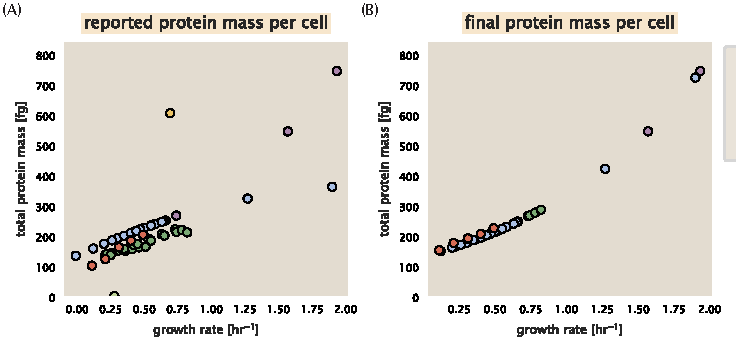
\includegraphics{SI_figs/dataset_corrections.pdf}
        \caption{\textbf{Summary of the growth-rate dependent total protein
        abundance for each data set.} (A) Total protein abundance per cell as
        originally reported in the data sets of \cite{taniguchi2010, valgepea2013, li2014,
        soufi2015, peebo2015, schmidt2016}. Note that the data from \cite{peebo2015} only
        reported protein abundances per unit volume and total protein per cell
        was found by multiplying these by the growth-rate dependent cell size as
        determined by \cite{si2017}. (B) Adjusted total protein abundances
        across the proteomic data sets are summarized. Protein abundances were
        adjusted so that all data shared a common set of growth-rate dependent
        total protein per cell and cellular protein concentration following the
        cell size expectations of \cite{si2017} (see section on
        \nameref{sec:protein_size_SV} for further details). }
        \label{fig:total_protein_final}
    }
    \end{fullwidth}
\end{figure}

Lastly, in \FIG{venn} we show the total proteomic coverage and overlap of
proteins quantified across each data set. In part (A) we plot the total number
of  unique proteins, while in part (B) we plot a Venn diagram to also show the
intersections across each data set. Overall, the overlap in quantified proteins
is quite high, with 1157 proteins quantified across all data sets. The
sequencing based approach of \cite{li2014} has substantially higher coverage
compared to the mass spectrometry data sets (3394 genes versus the 2041 genes
quantified in the work of \cite{schmidt2016}). However, in terms of total
protein mass, the data from \cite{li2014, schmidt2016, peebo2015} each quantify
roughly equivalent total protein mass.  An exception to this is in the data from
\cite{valgepea2013}, where we find that  the total protein quantified in
\cite{valgepea2013} is 90-95 \% of the total protein mass (when using the data
from \cite{schmidt2016} as a reference).


% \begin{figure*}
%     \centering{
%         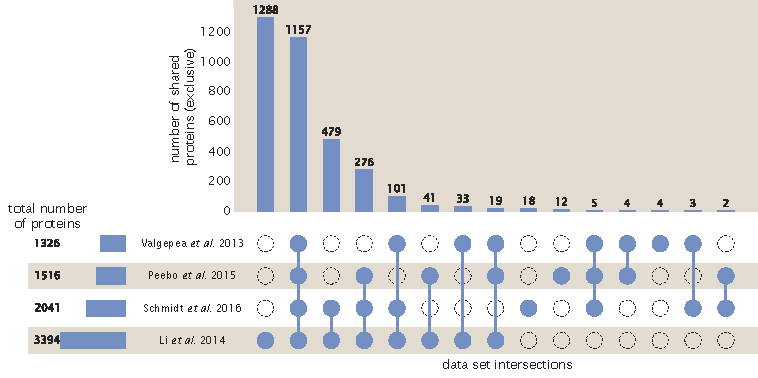
\includegraphics{SI_figs/dataset_upset_diagram.pdf}
%         \caption{\textbf{Comparison of proteomic coverage across different data sets.}
%         An UpSet diagram \citep{Lex2014} summarizes the total number of protein
%         coding genes whose protein abundance was reported in the data sets of
%         \cite{valgepea2013, li2014, schmidt2016, peebo2015}. Bar plot on bottom
%         left indicates the total number of genes reported in each individual
%         data. The main bar plot summarizes the number of unique proteins
%         identified across overlapping subsets of the data.  For example, in the
%         first column only the data from \cite{li2014}  is considered (indicated
%         by solid blue circle) and 1288 proteins are identified as exclusive to
%         the data set. In the second column, the intersection of all four data
%         sets is considered, with 1157 proteins quantified across them. This
%         follows for each additional column in the plot, with the subset under
%         consideration denoted by the solid blue circles.
%         } \label{fig:upset}
%     }
% \end{figure*}

\begin{figure*}
    \centering{
        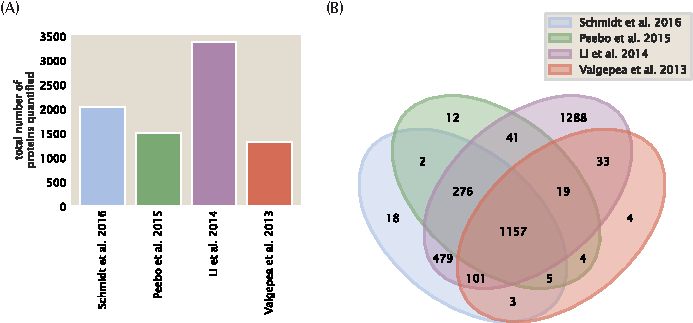
\includegraphics{SI_figs/intersections_venn.pdf}
        \caption{\textbf{Comparison of proteomic coverage across different data sets.}
        (A) Total number of unique proteins quantified in the data sets of
        \cite{valgepea2013, li2014, schmidt2016, peebo2015}. (2) Venn diagram
        showing the number of unique proteins and their intersections across each
        of the four data sets in (A). The intersection of all four data
        sets identifies 1157 proteins with measured protein copy number values.
        } \label{fig:venn}
    }
\end{figure*}

\section{Estimation of Cell Size and Surface Area}
\label{sec:protein_size_SV}
Since most of the proteomic data sets lack cell size (i.e. volume) measurements, we chose
instead to use a common estimate of size for any analysis requiring cell
size or surface area.  Since each of the data sets used either K-12 MG1655 or
its derivative, BW25113 (from the lab of Barry L. Wanner; the parent strain of
the Keio collection \citep{datsenko2000, baba2006}), we fit the MG1655 cell size
data from the supplemental material of \cite{si2017, si2019} using the optimize.curve\_fit function
from the Scipy python package \citep{2020scipynmeth}.

The average size measurements from each of their experiments are shown in Figure
\FIG{final_size_data_Si}, with  cell length and width shown in (A) and (B),
respectively. The length data was well described by the exponential function 0.5
$e^{1.09 \cdot \lambda}$ + 1.76 \textmu m, while the width data was well
described by 0.64 $e^{0.24 \cdot \lambda}$ \textmu m. In order to estimate cell
size we take the cell as a cylinders with two hemispherical ends \citep{si2017,
basan2015}. Specifically,  cell size  is estimated from,

\begin{equation}
V = \pi \cdot r^2 \cdot (l - 2r/3),
\label{eq:cell_size}
\end{equation}
where $r$ is half the cell width. A best fit to the data is described by 0.533
$e^{1.037 \cdot \lambda}$ \textmu m$^3$. Calculation of the cell surface area is
given by,

\begin{equation}
 S = \eta \cdot \pi (\frac{\eta \cdot \pi}{4} - \frac{\pi}{12})^{-2/3} V^{2/3},
 \label{eq:surface_area}
\end{equation}
where $\eta$ is the aspect ratio ($\eta$ = $l/w$) \citep{ojkic2019}.

\begin{figure}
		\centering
    \includegraphics[width=1.0\textwidth]{SI_figs/Si_size_data_fit.pdf}
    \caption{\textbf{Summary of size measurements from Si \textit{et al.} 2017,
    2019.} Cell lengths and widths were measured from cell contours obtained from
    phase contrast images, and refer to the long and short axis respectively. (A)
    Cell lengths and (B) cell widths show the mean measurements reported (they
    report 140-300 images and 5,000-30,000 for each set of samples; which likely
    means about 1,000-5,000 measurements per mean value reported here since they
    considered about 6 conditions at a time). Fits were made to the  MG1655 strain
    data; length: 0.5 $e^{1.09 \cdot \lambda}$ + 1.76 \textmu m, width:  0.64
    $e^{0.24 \cdot \lambda}$ \textmu m. (C) Cell size, $V$, was calculated as
    cylinders with two hemispherical ends (Equation \ref{eq:cell_size}). The
    MG1655 strain data gave a best fit of 0.533 $e^{1.037 \cdot \lambda}$ \textmu m$^3$.}
  \label{fig:final_size_data_Si}
\end{figure}


\section{Estimation of Total Protein Content per Cell}
\label{sec:estimate_protein_per_cell}
In order to estimate total protein per cell for a particular growth rate, we
begin by estimating the cell size from the fit shown in Figure
\FIG{final_size_data_Si}(C) (0.533 $e^{1.037 \cdot \lambda}$ \textmu m$^3$). We
then estimate the total protein content from the total dry mass of the cell.
Here we begin by noting that  for almost the entire range of growth rates
considered here, protein, DNA, and RNA were reported to account for at least 90
\% of the dry mass (\cite{basan2015}). The authors also found that the total dry
mass concentration was roughly constant across growth conditions. Under such a
scenario, we can calculate the total dry mass concentration for protein, DNA,
and RNA, which is given by 1.1 g/ml x 30 \% x 90 \% or about $[M_P]$ = 300 fg
per fl. Multiplying this by our prediction of cell size gives the total dry mass
per cell.

However, even if dry mass concentration is relatively constant across growth
conditions, it is not obvious how protein concentration might vary due to
the substantial increase in rRNA at faster
growth rates (\cite{dai2016}). This is a well-documented result that arises from
an increase in ribosomal abundance at faster growth rates
(\cite{scott2010}). To proceed therefore rely on experimental
measurements of total DNA content per cell that also come from Basan \textit{et
al.}, and RNA to protein ratios that were measured in Dai \textit{et al.} (and
cover the entire range of growth conditions considered here). These are
reproduced in Figure \FIG{schmidt_adjustment_varying_conc}(A) and (B),
respectively.

Assuming that the protein, DNA, and RNA account for 90 \% of the total dry mass,
the protein mass can then determined by first subtracting the experimentally
measured DNA mass,  and then using the experimental estimate of the RNA to
protein ratio. The total protein per cell is will be related to the summed RNA
and protein mass by,

\begin{equation}
	M_{P} = \frac{[M_P + M_{RNA}]}{1 + (RP_{ratio})}.
\end{equation}
$(RP_{ratio}$ refers to the RNA to protein ratio as measured by Dai \textit{et
al.}. In Figure \FIG{schmidt_adjustment_varying_conc}(C) we plot the estimated
cellular concentrations for protein, DNA, and RNA from these calculations, and
in Figure \FIG{schmidt_adjustment_varying_conc}(D) we plot their total expected
mass per cell. This later quantity is the growth rate-dependent total protein
mass that was used to estimate total protein abundance across all data sets (and
summarized in \FIG{total_protein_final}(B)).


\begin{figure}
		\centering
    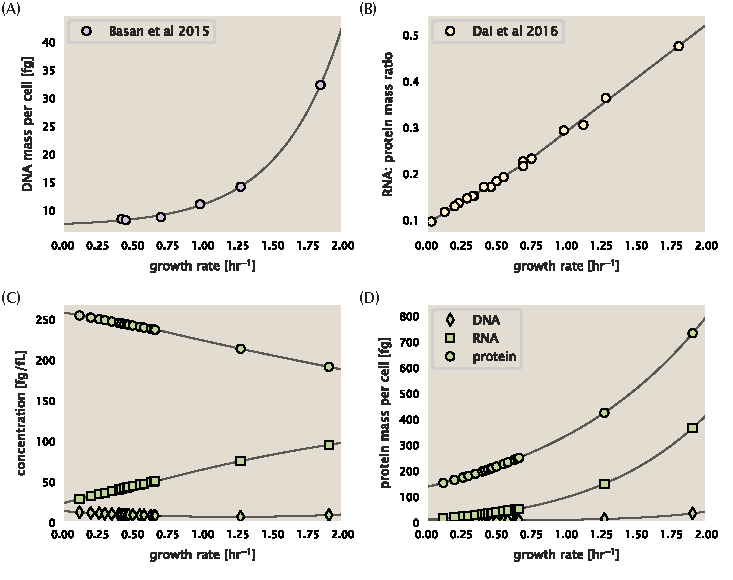
\includegraphics[width=1\textwidth]{SI_figs/schmidt_estimate_protein_RNA_DNA_corrections.pdf}
  \caption{{\bf Empirical estimate of cellular protein, DNA, and RNA as a
  function of growth rate.} (A) Measured DNA mass per cell as a function of
  growth rate, reproduced from Basan \textit{et al.} 2015. The data was fit to
  an exponential curve (DNA mass in fg per cell is given by 0.42 $e^{2.23 \cdot
  \lambda}$ + 7.2 fg per cell, where $\lambda$ is the growth rate in hr$^{-1}$).
  (B) RNA to protein measurements as a function fo growth rate. The data was for
  to two lines: for growth rates below 0.7 hr$^{-1}$, the RNA/protein ratio is
  0.18$\cdot \lambda$ + 0.093, while for growth rates faster than 0.7 hr$^{-1}$
  the RNA/protein ratio is given by 0.25$\cdot \lambda$ + 0.035. For (A) and (B)
  cells are grown under varying levels of nutrient limitation, with cells grown
  in minimal media with different carbon sources for the slowest growth
  conditions, and rich-defined media for fast growth rates. (C) Predictions of
  cellular protein, DNA, and RNA concentration.  (D) Total cellular mass
  predicted for protein, DNA, and RNA using the cell size predictions from Si
  \textit{et al.}. Symbols (diamond: DNA, square: RNA, circle: protein)
	show estimated values of mass concentration and mass per cell for the specific
	growth rates in \cite{schmidt2016}.
	 	}
  \label{fig:schmidt_adjustment_varying_conc}
\end{figure}

\subsection{Estimating Volume and Number of Amino Acids from Ribosome Copy Number}
Towards the end of the main text, we examine a coarse-grained model of
nutrient-limited growth. A key point in our analysis was to consider  how
elongation rate $r_t$ and growth rate $\lambda$ vary with respect to the
experimentally observed changes in cell size, total number of peptide bonds per
cell  $N_\text{pep}$, and ribosomal content.  In order to do maintain parameters
in line with the experimental data, but otherwise allow us to explore the
model, we performed a phenomenological fit of $N_\text{pep}$ and $V$ as a
function of the measured ribosomal copy number $R$. As has been described in the
preceding sections of this supplement, we estimate cell volume for each growth
condition using the size measurements from \cite{si2017,si2019}, and
$N_\text{pep}$ is approximated by taking the total protein mass and dividing
this number by the average mass of an amino acid, 110 Da (BNID: 104877).

Given the  exponential scaling of $V$ and $N_\text{pep}$ with growth rate,
we performed a linear regression of the log transform of these parameters
as a function of the log transform of the ribosome copy number. Using
optimization by minimization, we estimated the best-fit values of the intercept
and slope for each regression. \FIG{naa_v_fit} shows the result of each
regression as a dashed line, given in terms of the linear-scaled data.

\begin{figure}
  \centering{
    \includegraphics{SI_figs/log_log_resgression_naa_vol.pdf}
    \caption{\textbf{Phenomenological regression of cell volume and number of
    amino acids per cell as a function of the ribosome copy number.} Colored
    points correspond to the measured value (or calculated value in the case of
    the cell volume) with colors denoting different data sets. The dashed black
    line shows the result of the fit, with the functional form of the equation
    given in the legend with $R$ representing the ribosome copy number.}
  }
\end{figure}

\input{SI_section_03_schmidt.tex}
\section{Calculation of Complex Abundance}

All protein data quantified the abundance of individual proteins per cell.
However, this work requires estimates on the abundance of individual protein
\textit{complexes}, rather than the copy number of individual proteins. In our
analysis of the protein copy number data, it became clear that the reported copy
numbers do not always align with those based on reported stiochometry. As one
example of this, the F-O subunit of ATP synthase consists of three protein
subunits with a stoichiometry of [AtpB][AtpF]$_2$[AtpE]$_{10}$ (also referred to
as subunits a, b, and c, respectively). In the experimental data of
\cite{schmidt2016}, the values deviate from this quite substantially, with
approximately 1000 AtpB, 9000 AtpF, and 300 AtpE reported per cell (minimal
media + glucose growth condition).  This highlights the technical challenges
that still remain in our ability to quantify cellular composition, particularly
for membrane-bound proteins like the ATP synthase complex considered here.  In
this section, we outline the approach we used to annotate proteins as part of
each macromolecular complex and how we used averaging across the individual
protein measurements to estimate an absolute complex abundances per cell.

Protein complexes, and proteins individually, often have a variety of names,
both longform and shorthand. As individual proteins can have a variety of
different synonyms, we sought to ensure that each protein annotated in the
data sets used the same synonym. To do use, we relied heavily on the EcoCyc
Genomic Database \citep{keseler2017}.  Each protein in available data sets
included an annotation of one of the gene name synonyms as well as an
accession ID -- either a UniProt or Blattner "b-number". We programmatically
matched up individual accession IDs between the proteins in different data sets.
In cases where accession IDs matched but the gene names were different, we
manually verified that the gene product was the same between the datasets and
chose a single synonym.  All code used  in the data cleaning and unification
procedures can be found on the associated
\href{https://github.com/rpgroup-pboc/growth_limits}[GitHub repository]
(DOI:XXX) associated with this paper as well as on the associated
\href{https://rpgroup.caltech.edu/growth_limits}{paper website}.

With each protein conforming to a single identification
scheme, we then needed to identify the molecular complexes each protein was a
member of. Additionally, we needed to identify how many copies of each protein
were present in each complex (i.e. the subunit copy number) and compute the
estimated abundance complex that accounted for fluctuations in subunit
stoichiometry. To map proteins to complexes, we accessed the
EcoCyc \textit{E. coli} database \cite{keseler2017} using PathwayTools version
23.0 \cite{karp2019}. With a license for PathWay Tools, we
mapped each unique protein to its annotated complexes via the
BioCyc Python package. As we mapped each protein with \textit{all} of its
complex annotations, there was redundancy in the dataset. For example, ribosomal
protein L20 (RplT) is annotated to be a component of the 50S ribosome (EcoCyc
complex \texttt{CPLX-03962}) as well as a component of the mature 70S ribosome
(EcoCyc complex \texttt{CPLX-03964}).

In addition to the annotated complex, we collected information on the
stoichiometry of each macromolecular complex. For a complex with $N_\text{subunits}$ protein species,
for each protein subunit $i$ we first calculate the number of complexes that
\textit{could} be formed given the measured protein copy numbers per cell,
\begin{equation}
    N_\text{complex}(\text{subunit i}) = \frac{P_\text{subunit i}^\text{(measured)}}{m_\text{subunit i}}.
    \label{eq:subunit_max}
\end{equation}
Here, $P_\text{subunit i}^\text{(measured)}$ refers to the measured protein copy number of species $i$,
and $m$ refers to the number of monomers present for that protein in the complex. For example, the 70S mature ribosome complex has 55 protein components, all of
which are present in a single copy except L4 (RplL), which is present in 4
copies ($m$ = 4). For each ribosomal protein, we then calculate the  maximum number of
complexes that could be formed using Equation \ref{eq:subunit_max}. This example, along with
example from 5 other macromolecular complexes, can be seen in
Figure \ref{fig:complex_counting}.

It is important to note that measurement noise, efficiency of protein
extraction, and differences in protein stability will mean that the precise value of each
calculation will be different for each component of a given complex. Thus, to
report the total complex abundance, we use the arithmetic mean of
across all subunits in the complex,
\begin{equation}
   \langle N_\text{complex} \rangle = \frac{1}{N_\text{subunits}}\sum\limits_i^{N_\text{subunits}} \frac{P_{i}^\text{(measured)}}{m_\text{subunit i}}.
   \label{eq:complex_count}
\end{equation}
in Figure \ref{fig:complex_counting}, we show this mean value as a grey line for a variety
of different complexes. Additionally, we have built an interactive figure
accessible on the \href{https://www.rpgroup.caltech.edu/growth_limits}{paper
website} where the validity of this approach can be examined for any complex
with more than two subunits (thus, excluding monomers and dimers).

\begin{figure}
        \centering{
            \includegraphics{SI_figs/figS10_subunit_counting.pdf}
            \caption{\textbf{Calculation of the mean complex abundance from
            measurements of single subunits.} Six of the largest complexes (by
            number of subunits) in \textit{E. coli}. Points correspond to the
            maximum number of complexes that can be formed given measurement of
            that individual protein. Solid grey line corresponds to the
            arithmetic mean across all subunits. These data correspond to
            measurements from \cite{schmidt2016} in a glucose-supplemented
            minimal growth medium.}
            \label{fig:complex_counting}
        }
\end{figure}

\section{Extending Estimates to a Continuum of Growth Rates}
\label{sec:SI_continuum_est}
In the main text, we considered a standard stopwatch of 5000 s to estimate the
abundance of the various protein complexes considered. In addition to point
estimates, we also showed the estimate as a function of growth rate as
transparent grey curves. In this section, we elaborate on this continuum
estimate, giving examples of estimates that scale with either cell volume, cell
surface area, or number of origins of replication.

\subsection{Estimation of the total cell mass}
For many of the processes estimated in the main text we relied on a cellular dry
mass of $\approx 300$ fg from which we computed elemental and protein fractions
using knowledge of fractional composition of the dry mass. At modest growth
rates, such as the 5000 s doubling time used in the main text, this is a
reasonable number to use as the typical cell mass is $\approx$ 1 pg and
\textit{E. coli} cells can approximated as 70\% water by volume. However, as we
have shown in the preceding sections, the cell size is highly dependent on the growth rate. This means that a dry mass of 300
fg cannot be used reliably across all growth rates.

Rather, using the phenomenological  description of cell volume scaling
exponentially with growth rate, and using a rule-of-thumb of a cell buoyant
density of $\approx 1.1$ pg / fL (BNID: 103875), we can calculate the cell dry mass across a
range of physiological growth rates as
\begin{equation}
    m_\text{cell} \approx \rho V(\lambda) \approx \rho ae^{\lambda * b}
    \label{eq:def_mcell}
\end{equation}
where $a$ and $b$ are constants with units of \textmu m$^3$  and hr,
respectively. The value of these constants can be estimated from the careful
volume measurements performed by \cite{si2017}, as considered in Appendix \nameref{sec:protein_size_SV} earlier.

\subsection{Complex Abundance Scaling With Cell Volume}
Several of the estimates performed in the main text are implicitly dependent
on the cell volume. This includes processes such as ATP utilization and, most
prominently, the transport of nutrients, whose demand will be proportional to the volume
of the cell. Of the latter, we estimated the
number of transporters that would be needed to shuttle enough carbon,
phosphorus, and sulfur across the membrane to build new cell mass. To do so,
we used elemental composition measurements combined with a 300 fg cell dry
mass to make the point estimate. As we now have a means to estimate the total
cell mass as a function of volume, we can generalize these estimates across
growth rates.

Rather than discussing the particular details of each transport system, we will
derive this scaling expression in very general terms. Consider that we wish to
estimate the number of transporters for some substance $X$, which has been
measured to be made up some fraction of the dry mass, $\theta_X$. If we assume
that, irrespective of growth rate, the cell dry mass is relatively constant
\citep{basan2015} and $\approx$ 30\% of the total cell mass, we can state that
the total mass of substance $X$ as a function of growth rate is
\begin{equation}
m_X \approx 0.3 \times \rho V(\lambda) \theta_X,
\label{eq:m_x}
\end{equation}
where we have used $\rho V(\lambda)$ as an estimate of the total cell mass,
defined in Equation \ref{eq:def_mcell}. To convert this to the number of units $N_X$ of substance
$X$ in the cell, we can use the formula weight $w_X$ of a single unit of $X$ in
conjunction with Equation \ref{eq:m_x},
\begin{equation}
    N_X \approx \frac{m_X}{w_X}.
    \label{eq:n_x}
\end{equation}

To estimate the number of transporters needed, we make the approximation that
loss of units of $X$ via diffusion through porins or due to the permeability of
the membrane is negligible  and that a single transporter complex can transport
substance $X$ at a rate $r_X$. As this rate $r_X$  is in units of $X$ per time
per transporter, we must provide a time window over which the transport process
can occur. This is related to the cell doubling time $\tau$, which can be
calculated from the the growth rate $\lambda$ as $\tau = \log(2) / \lambda$.
Putting everything together, we arrive at a generalized transport scaling
relation of
\begin{equation}
N_\text{transporters}(\lambda) = \frac{0.3 \times \rho V(\lambda)\theta_X}{w_X r_X \tau}.
\label{eq:transporter_continuum}
\end{equation}

This function is used to draw the continuum estimates for the number of
transporters seen in Figures 2 and 3 as transparent grey curves. Occasionally,
this continuum scaling relationship will not precisely agree with the point
estimate outlined in the main text. This is due to the choice of $\approx$ 300 fg
total dry mass per cell for the point
estimate, whereas we considered more precise values of cell mass in the continuum estimate. We
note, however, that both this scaling relation and the point estimates are meant
to describe the order-of-magnitude observed, and not the predict the exact
values of the abundances.

Equation \ref{eq:transporter_continuum} is a very general relation for processes where the
cell volume is the "natural variable" of the problem. This means that, as the
cell increases in volume, the requirements for substance $X$ also scale with
volume rather than scaling with surface area, for example. So long as the rate
of the process, the fraction of the dry mass attributable to the substance, and
the formula mass of the substance is known, Equation \ref{eq:transporter_continuum} can be
used to compute the number of complexes needed. For example, to compute the
number of ATP synthases per cell, Equation \ref{eq:transporter_continuum} can be slightly
modified to the form
\begin{equation}
    N_\text{ATP synthases}(\lambda) = \frac{0.3 \times \rho V(\lambda)\theta_{protein}N_\text{ATP}}{w_{AA} r_\text{ATP} \tau},
\end{equation}
where we have included the term $N_\text{ATP}$ to account for the number of ATP
equivalents needed per amino acid for translation ($\approx$ 4, BNID: 114971),
and $w_{AA}$ is the average mass of an amino acid. The grey curves in Figure 4
of the main text were made using this type of expression.

\subsection{A Relation for Complex Abundance Scaling With Surface Area}
In our estimation for the number of complexes needed for lipid synthesis and
peptidoglycan maturation, we used a particular estimate for the cell surface
area ($\approx$ 5 \textmu$m$, BNID: 101792) and the fraction of dry mass
attributable to peptidoglycan ($\approx$ 3\%, BNID: 101936). Both of these
values come from glucose-fed \textit{E. coli} in balanced growth. As we are
interested in describing the scaling as a function of the growth rate, we must
also consider how these values scale with cell surface area, which is the natural
variable for these types of processes. In the coming paragraphs, we highlight
how we incorporate a condition-dependent surface area into our calculation of
the number of lipids and murein monomers that need to be synthesized and
crosslinked, respectively.

\subsubsection{Number of Lipids}
To compute the number of lipids as a function of growth rate, we make the
assumption that some features, such as the surface area of a single lipid
($A_\text{lipid} \approx$ 0.5 nm$^2$, BNID: 106993) and the total fraction of the membrane
composed of lipids ($\approx$ 40\%, BNID: 100078) are independent of the growth
rate. Using these approximations combined with Equation \ref{eq:surface_area}, and
recognizing that each membrane is composed of two leaflets, we can
compute the number of lipids as a function of growth rate as

\begin{equation}
    N_\text{lipids}(\lambda) \approx \frac{4\,\text{leaflets} \times 0.4 \times
    \eta\pi\left(\frac{\eta\pi}{4} -
    \frac{\pi}{12}\right)^{-2/3}V(\lambda)^{2/3}}{A_\text{lipid}}
\end{equation}
where $\eta$ is the length-to-width aspect ratio and $V$ is the cell volume.

\subsubsection{Number of Murein Monomers}
In calculation of the number of transpeptidases needed for maturation of the
peptidoglycan, we used an empirical measurement that $\approx$ 3\% of the dry
mass is attributable to peptidoglycan and that a single murien monomer is
$m_\text{murein} \approx$ 1000 Da. While the latter is independent of growth rate, the former is
not. As the peptidoglycan exists as a thin shell with a width of $w \approx 10$
nm encapsulating the cell, one would expect the number of murein monomers scales
with the surface area of this shell. In a similar spirit to our calculation of
the number of lipids, the total number of murein monomers as a function of
growth rate can be calculated as
\begin{equation}
N_\text{murein monomers}(\lambda) \approx \frac{\rho_\text{pg} w \eta\pi\left(\frac{\eta\pi}{4} -
    \frac{\pi}{12}\right)^{-2/3}V(\lambda)^{2/3}}{m_\text{murein}},
\end{equation}
where $\rho_\text{pg}$ is the density of peptidoglycan.


\subsection{Complex Abundance Scaling With Number of Origins, and rRNA Synthesis}
While the majority of our estimates hinge on the total cell volume or surface
area, processes related to the central dogma, namely DNA replication and
synthesis of rRNA, depend on the number of chromosomes present in the cell. As
discussed in the main text, the ability of \textit{E. coli} to parallelize the
replication of its chromosome by having multiple active origins of replication
is critical to synthesize enough rRNA, especially at fast growth
rates. Derived in \cite{si2017} and reproduced in the main text and Appendix \nameref{sec:SI_ori} below, the average number of
origins of replication at a given growth rate can be calculated as
\begin{equation}
\langle\# \text{ori} \rangle \approx 2^{t_\text{cyc} \lambda / \ln 2}
\label{eq:nori}
\end{equation}
where $t_\text{cyc}$ is the total time of replication and division. We can make
the approximation that $t_\text{cyc} \approx$ 70 min, which is the  time from
the initiation of chromosomal replication until division. This time corresponds to
the sum of the so-called C and D periods of the cell cycle, which correspond to
the time it takes to replicate the entire chromosome (C period) and the time
from completion to eventual division (D period) \cite{helmstetter1968}.

In the case of rRNA synthesis, the majority of the rRNA operons are surrounding
the origin of replication. Thus, at a given growth rate $\lambda$, the average
dosage of rRNA operons per cell $D_\text{rRNA}$ is
\begin{equation}
D_\text{rRNA}(\lambda) \approx N_\text{rRNA operons} \times 2^{t_{cyc} \lambda / \ln 2}.
\label{eq:rRNA_dosage}
\end{equation}

This makes the approximation that \textit{all} rRNA operons are localized around
the origin. In reality, the operons are some distance away from the origin,
making Equation \ref{eq:rRNA_dosage} an approximation \citep{dennis2004}.

In the main text, we stated that at a growth rate of 0.5 hr$^{-1}$, there is
$\approx$ 1 chromosome per cell. While a fair approximation, Equation \ref{eq:nori}
illustrates that is not precisely true, even at slow growth rates. In estimating
the number of RNA polymerases as a function of growth rate, we consider that
regardless of the number of rRNA operons, they are all sufficiently loaded with
RNA polymerase such that each operon produces one rRNA per second. Thus, the
total number of RNA polymerase as a function of the growth rate can be
calculated as
\begin{equation}
    N_\text{RNA polymerase}(\lambda) \approx L_\text{operon}D_\text{rRNA}\rho_\text{RNA polymerase},
\end{equation}
where $L_\text{operon}$ is the total length of an rRNA operon ($\approx$ 4500
bp) and $\rho_\text{RNA polymerase}$ is packing density of RNA polymerase on a
given operon, taken to be 1 RNA polymerase per 80 nucleotides.


\section{Calculation of active ribosomal fraction.}
\label{sec:SI_f_a}
In the main text we used the active ribosomal fraction $f_a$ that was reported
in the work of \cite{dai2016} to estimate the active ribosomal mass fraction
$\Phi_R \times f_a$ across growth conditions. We lacked any specific model to
consider how  $f_a$ should vary with growth rate, and instead find that the data
is well-approximated by fitting to an exponential curve ($f_a$ = -0.889 $e^{4.6
\cdot \lambda}$ + 0.922; dashed line in inset of \textbf{\textit{Figure 10}}(C)). We
use this function to estimate $f_a$ for each of the data points shown in
 \textbf{\textit{Figure 10}}(C).

\section{Estimation of $\langle$\#ori$\rangle$ / $\langle$\#ter$\rangle$ and $\langle$\#ori$\rangle$.}
\label{sec:SI_ori}
\textit{E. coli} shows robust scaling of cell size with the average number
of origins per cell, $\langle$\#ori$\rangle$ \citep{si2017}. Since protein makes
up a majority of the cell's dry mass, the change in cell size is also a
reflection of the changes in proteomic composition and total abundance across
growth conditions. Given the potential constraints on rRNA synthesis and changes
in ribosomal copy number with $\langle$\#ori$\rangle$, it becomes important to
also consider how protein copy numbers vary with the state of chromosomal
replication. This is particularly true  when trying to make sense of the changes
in ribosomal fraction and growth-rate dependent changes in proteomic composition
at a  mechanistic level.  As considered in the main text, it is becoming
increasingly apparent that regulation through the secondary messengers (p)ppGpp
may act to limit DNA replication and also reduce ribosomal activity in poorer
nutrient conditions.  In this context, both $\langle$\#ori$\rangle$, as well as
the $\langle$\#ori$\rangle$ / $\langle$\#ter$\rangle$ ratio become important
parameters to consider and keep track of. An increase in $\langle$\#ori$\rangle$
/ $\langle$\# ter$\rangle$ ratio  in particular, causes a relatively higher gene
dosage in rRNA and r-protein genes due to skew in genes near the origin, where
the majority of these are located

In the main text we estimated the change in $\langle$\#ori$\rangle$ with growth
rate using the nutrient-limited wild-type cell data from \cite{si2017}. We
consider their measurements of DNA replication time ($t_{C}$, 'C' period of
cell division), total cell cycle time ($t_{cyc}$, 'C' + 'D' period of cell
division), and doubling time $\tau$ from wild-type \textit{E. coli} growing
across a range of growth conditions. Here we show how we  esimate this
parameter, as well as the $\langle$\#ori$\rangle$ / $\langle$\# ter$\rangle$
ratio from their data.  We begin by considering $\langle$\#ori$\rangle$. If the
cell cycle time takes longer  than the time of cell division, the cell will need
to initiate DNA replication  more often than its rate of division, $2^{\lambda
t} = 2^{ln(2) \cdot t/ \tau}$ to maintain steady state growth. Cells will need
to do this in proportion to the ratio $\lambda_{cyc} / \lambda =  t_{cyc}/\tau$,
and the number of origins per cell (on average) is then given by $2^{t_{cyc}/
\tau}$.   The average number of termini will in contrast depend on the lag time
between  DNA replication and cell division, $t_{D}$, with
$\langle$\#ori$\rangle$ / $\langle$\# ter$\rangle$ ratio = $2^{t_{cyc}/ \tau -
t_{D}/ \tau} =  2^{t_{C}/ \tau}$.

In Figure \ref{fig:Si_tC_tcyc}(A) and (B) we plot the measured $t_{C}$ and $t_{cyc}$
values versus the doubling time from \cite{si2017}. The authors estimated
$t_{C}$ by marker frequency analysis using qPCR, while  $t_{cyc} = t_{C} +
t_{D}$ were inferred from $t_{C}$ and $\tau$. In the plots we see that both
$t_{C}$ and $t_{cyc}$ reach a minimum  at around 40 and 75 minutes,
respectively. For a C period of 40 minutes, this would correspond to a maximum
rate of elongation of about 1,000 bp/sec. Since we lacked a specific model to
describe how each of these parameters vary with growth condition, we assumed
that they were linearly dependent on the doubling time. For each parameter,
$t_{C}$ and $t_{cyc}$, we split them up into two domains corresponding to poorer
nutrient conditions and rich nutrient conditions (cut off at $\tau \approx$ 40
minutes where chromosomal replication becomes nearly constant). The fit lines
are shown as solid black lines. In Figure \ref{fig:Si_tC_tcyc}(C) and (D) we also
show $t_{C}$ and $t_{cyc}$ as a function of growth rate $\lambda$ along with our
piecewise linear fits, which match the plots in the main text.


\begin{figure}
    \begin{fullwidth}
        \centering{
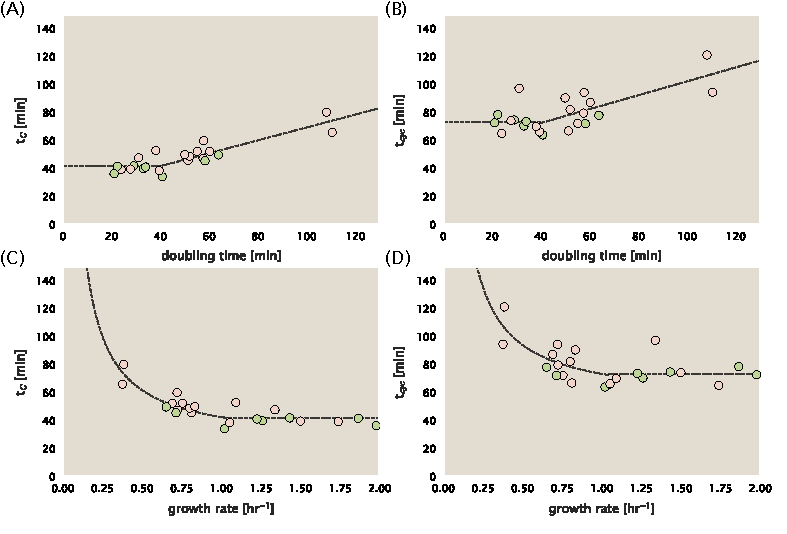
\includegraphics{SI_figs/figA10_ori_ter.pdf} \caption{\textbf{Estimation of
    $\langle$\#ori$\rangle$ / $\langle$\# ter$\rangle$ and
    $\langle$\#ori$\rangle$ using data from Si \textit{et al.} (2017).} (A) and
    (B) plot the reported $t_{C}$ and $t_{cyc}$ as a function  of cell doubling
    time $\tau$, respectively. The dashed lines show a piecewise fit to  the
    data. For short doubling times (rich media), $t_{C}$ and $t_{cyc}$ are
    assumed  constant ($t_{C}$ = 42 minutes, $t_{cyc}$ = 73 minutes). At the transition, taken to occur at 40 minutes, the
    dashed line corresponds  to an assumed proportional increase in each
    parameter as a function of the doubling time ($t_{C}$ = 0.46 $\tau$ + 23.3 minutes,
    $t_{cyc}$ = 0.50 $\tau$ + 52.7 minutes). (C) and (D) plot the same data
    as in (A) and (B), but as a function of growth rate, given by $\lambda = ln(2)/\tau$.}
\label{fig:Si_tC_tcyc} }
\end{fullwidth}
\end{figure}

\section{Derivation of Minimal Model for Nutrient-Mediated Growth Rate Control}
\label{sec:SI_model}
Here we provide a derivation of the minimal model for growth rate control under
nutrient-limited growth. By growth rate control, we are specifically referring
to the ability of bacteria to modulate their proteome ($N_\text{pep}$, $R$,
$\Phi_R$) and cell size as nutrient conditions change, with slower growing cells
generally being smaller in size \citep{ojkic2019}. This capability provides
bacteria with  a particular benefit when nutrients are more scarce since it will
mean there is a  smaller net demand on carbon, phosphorus, sulfur, and nitrogen.
The specific goal  of developing this model is to help us better explore the
overall constraints on  growth that follow from 1) our observation that many  of
the cellular processes we've considered require increased protein abundance at
faster growth rates, and 2) a strict limit on growth rate that is
governed by the ribosomal synthesis rate and ribosomal mass fraction $\Phi_R$.

In \textbf{\textit{Figure 12}}(A) of the main text we provide a schematic of the
model, where we consider growth as simply governed by the rate of protein
synthesis ($r_t \times R \times f_a$). In order to grow rapidly, at least to the
extent possible, these three parameters need to be maximized (with $r_t \leq$ 17
amino acids per second, and $f_a \leq$ 1 reported in the work of
\cite{dai2016}). The elongation rate $r_t$ will depend on how quickly
ribosomes can match codons with their correct amino-acyl tRNA, along with the
subsequent steps of peptide bond formation and translocation. This ultimately
depends on the cellular concentration amino acids, which we treat as a single
effective species, $[AA]_\text{eff}$.

In our model, we need to determine the rate of peptide elongation $r_t$, which we
consider as simply depending on the supply of amino acids (and,
therefore, also amino-acyl tRNAs) through a parameter $r_{AA}$ in units of AA
per second, and the rate of amino acid consumption by protein synthesis ($r_t
\times R \times f_a$). The balance between these two rates will determine the
effective amino acid concentration in the cell $[AA]_\text{eff}$. An important
premise for this formulation is growing evidence that cells are able to modulate
their biosynthesis activity according to nutrient availability (i.e. extent of
chromosomal replication, transcriptional, and translation activity) through
secondary-messenger molecules like (p)ppGpp \citep{hauryliuk2015, zhu2019,
kraemer2019, fernandezcoll2020, Buke2020}. Given our observation that protein
synthesis and energy production are not limiting, we assume that other molecular
players required by ribosomes like elongation factors and GTP are available in
sufficient abundance. In addition, experimentally, the relative number of tRNA
and elongation factor EF-Tu per ribosome have been found to increase in poorer
nutrient conditions \cite{pedersen1978, dong1996, klumpp2013}).

We begin by considering a coarse-grained description of peptide elongation,
which includes 1) the time required to find and bind each correct amino-acyl
tRNA, and 2) the remaining steps in peptide elongation that will not depend on
the amino acid availability. These time scales will be related to the inverse of the
elongation rate $r_t$,

\begin{equation}
\frac{1}{r_t} = \frac{1}{k_{on} \alpha [AA]_{\text{eff}}} + \frac{1}{r_{t}^{\text{max}}}.
\end{equation}
where we have assumed that the rate of binding by amino-acyl tRNA $k_{on}$ is
proportional to $[AA]_{\text{eff}}$ by a constant $\alpha$. $r_{t}^{\text{max}}$
refers to the maximum elongation rate. This leads to a Michaelis-Menten
dependence of the elongation rate $r_t$ on the effective amino acid
concentration $[AA]_{\text{eff}}$ \citep{klumpp2013, dai2016}.
We can re-write this more succinctly in terms of an effective dissociation
constant,

\begin{equation}
    K_D = \frac{r_{t}^{\text{max}}}{\alpha k_\text{on}},
\end{equation}
where the elongation rate $r_t$ is now given by

\begin{equation}
r_t = \frac{r_{t}^{\text{max}}}{1 + K_D/[AA]_{\text{eff}}}.
\label{eq:rt_kd_simple}
\end{equation}

The rate of amino acid supply $r_{AA}$ will vary with changing nutrient
conditions and the cell can maintain $[AA]_{\text{eff}}$ by tuning the rate of
amino acid consumption, $r_t \times R \times f_a$.  Thus, $[AA]_{\text{eff}}$ is
determined by the difference in the rate of amino acid synthesis (or import, for
rich media) and/or tRNA charging,  $r_{AA}$, and the rate of consumption,
$r_t\times R \times f_a$. Over an  arbitrary length of time $t$ of cellular
growth, the cell will grow in volume, requiring us to consider these rates in
terms of concentration rather than absolute numbers, with $[AA]_{\text{eff}}$
given by,

\begin{equation}
\int_{0}^{t} \frac{d[AA]_{\text{eff}}}{dt} dt =  \int_{0}^{t}([r_{AA}] - [r_t\times R \times f_a]) dt.
\label{eq:aaeff_int}
\end{equation}
This considers the net change in amino acid concentration over a time from 0 to
$t$, with the square brackets indicating concentrations per unit time.
Integrating \EQ{aaeff_int} yields.
\begin{equation}
[AA]_{\text{eff}} =  t([r_{AA}] - [r_t \times R \times f_a]).
\label{eq:aaeff_concs}
\end{equation}

Alternatively, to connect to the experimental data in terms of absolute ribosome
copy number $R$ we can consider a unit volume $V$,
\begin{equation}
   [AA]_\text{eff} = \frac{t(r_{AA} - r_t \times R \times f_a)}{V \times N_A},
   \label{eq:aa_final}
\end{equation}
where $r_{AA}$ is in units of AA per unit time and $r_t$ is in units of AA per
unit time per ribosome. $N_A$ refers to Avogadro's number and is needed to
convert between  concentration and absolute numbers per cell. With an expression
for $[AA]_\text{eff}$ in hand, we can now solve \EQ{rt_kd_simple} for $r_t$
which is a quadratic function with a physically-meaningful root of

\begin{equation}
r_t = \frac{t(r_{AA} + r_t^\text{(max)}Rf_a) + K_D V N_A - \sqrt{(r_{AA}t + r_t^\text{(max)}Rf_at + K_D V N_A)^2 - 4(Rf_at)(r_t^\text{(max)}r_{AA} t)}}{2Rf_at}.
\label{eq:rt_root}
\end{equation}
This is the key equation that allows us to calculate growth rate for any
combination of $N_\text{pep}$, $R$, $f_a$, and cell size $V$ as a function of
amino acid supply $r_{AA}$ ( \textbf{\textit{Equation 3}}  of the main text). We refer the
reader to Section "A Minimal Model of Nutrient-Mediated Growth Rate Control " of the main text for our exploration of this
model in the context of the proteomic data.

We end this section by noting several distinctions of this formulation with
previous work. The first, as noted in the main text, relates to the now seminal
work of \cite{scott2010}, which provides a treatment of resource allocation that
partitions of the proteome into sectors -- including one for ribosome-associated
proteins and one for metabolic proteins. As cells grow faster, there is a
notable change in the mass fraction of these sectors, with an increase in
ribosomal content that is predominantly achieved at the expense of a decrease in
the metabolic sector. By including an additional constraint through the
phenomenological parameter $\nu$,  which characterizes the quality of the growth
medium \cite{scott2010, klumpp2013, klumpp2014}, the authors derive a model of
growth rate, dependent on optimal resource allocation. Here we have developed a
model that considers the effect of changes in absolute protein abundance and
ribosomal content, and consider how these influence the achievable growth rate.
In addition, by accounting for the metabolic supply of amino acids directly
though their availability in the cell (i.e. $[AA]_\text{eff}$), we are able to
consider how the balance between translation-specific metabolic capacity and
translational capacity influences both the elongation rate $r_t$ and growth
rate $\lambda$.

The second and last point we note is that the recent works from \cite{dai2016}
and \cite{klumpp2013} also employ a similar coarse-graining of translation
elongation as we've considered above. Here, however, a notable distinction is
that the authors consider the entire ternary complex (i.e. the complex of
amino-acyl tRNA, EF-Tu, and GTP) as rate limiting. Further, through an assumed
proportionality between ternary complex and ribosome abundance, they arrive at a
formulation of elongation rate $r_t$ that exhibits a Michaelis-Menten
dependence on the ribosomal fraction $\Phi_R$. They demonstrate that all their
measurements of elongation rate, even upon addition of sublethal doses of
chloramphenicol (which cause an increase in both $r_t$ and $\Phi_R$), can be
collapsed onto a single curve described by this Michaelis-Menten dependence.
There is always a benefit to increase their ribosomal fraction $\Phi_R$ on
growth rate when nutrient conditions allow (see Section "Maximum Growth Rate is Determined by the Ribosomal Mass Fraction" on the main text), and this trend
in the data in part follows from the tendency for cells to increase $\Phi_R$ and
better maximize $r_t$ as nutrient conditions improve.  In addition, it does not
account for the decrease in the fraction of actively translating ribosome $f_a$
that was strikingly apparent at slow growth rates or in sublethal doses of
chloramphenicol in the work of \cite{dai2016}. Through \EQ{rt_root} we also
account for changes in the fraction of actively translating ribosomes.
Ultimately, we find that cells are able to maximize both $\Phi_R$, $r_t$, and
their growth rate  only to the extent allowed by the nutrient conditions (i.e.
via $r_{AA}$) and through the maintenance of the cellular pool of amino acids
$[AA]_\text{eff}$, amino-acyl tRNA, GTP, as well as the synthesis of other key
molecular constituents like EF-Tu.


\bibliography{library}
\end{document}